\chapter{Entry Vehicle and Environment Models}\label{Ch:Models}
In this chapter we present the models of the entry vehicle and Mars environment used in the development and assessment of the entry guidance algorithm.
Vectors are denoted by boldface and are assumed to be columns. $(\cdot)^T$ denotes the transpose of a vector. 
The trace of a square matrix is the sum of its diagonal entries and is denoted $\trace(\cdot)$.   
%The gradient of a scalar function with respect to a vector is a row vector, i.e., $\mathbf{v}^T = \frac{\partial h(\y)}{\partial\y}$. 
The mean, or expected value, of a random variable, $\y$, is denoted by $\E{\y}=\bar{\y}$, and its covariance matrix by $\V{\y} = \cov_{\y}$. 
The standard deviation of a scalar random variable $y$ is $\sigma_{y} \triangleq \sqrt{\V{y}}$. A normal distribution with mean $\bar{\mathbf{y}}$ and covariance matrix $\cov_{\mathbf{y}}$ is $\normal(\bar{\mathbf{y}}, \cov_{\mathbf{y}})$.

\section{Three Degree-of-Freedom Dynamics Model}
The three degree-of-freedom translational dynamics for a Mars entry vehicle are defined relative to a Mars-fixed coordinate frame. In this three degree-of-freedom modeling, we have assumed that the velocity frame and the body frame are aligned, and do not consider the vehicle attitude.
% Talk about different independent variables, reduced longitudinal state vector 
The dynamics of an entry vehicle in an atmosphere are modeled by Vinh's equations \cite{VinhDyanmics}:
\begin{align}
	\dot{r} &= v\sin\gamma \label{Eq:dynamics:radius:time}\\
	\dot{\theta} &= \frac{v}{r}\frac{\cos\gamma\cos\psi}{\cos\phi} \\
	\dot{\phi} &= \frac{v}{r}\cos\gamma\sin\psi \\
	\dot{v} &= -D - g\sin\gamma \\ 
	\dot{\gamma} &= \frac{L}{v}\cos\sigma + \left(\frac{v}{r}-\frac{g}{v}\right)\cos\gamma + C_{\gamma}\\
	\dot{\psi} &= -\frac{L}{v\cos\gamma}\sin\sigma - \frac{v}{r}\cos\gamma\cos\psi\tan\phi + C_{\psi}\label{Eq:dynamics:heading:time}
\end{align}
where $r$ is the distance from the center of Mars to the center of mass of the entry vehicle, and $\theta$ and $\phi$ are latitude and longitude, respectively; the velocity vector is defined by the magnitude of the planet-relative velocity, $v$, the flight path angle $\gamma$, and the heading angle angle $\psi$, defined counterclockwise from East. The bank angle, $ \sigma $, is the clockwise rotation angle between the lift vector and the vertical plane containing the velocity vector; thus $\sigma=0$ corresponds to the full lift-up orientation. 
The magnitude of the gravitational acceleration is $g=\mu/r^2$, and $\mu=42,828\, \mathrm{km}^3/\mathrm{s}^2$ is the gravitational constant of Mars. Mars is assumed to be a sphere with planet radius $r_p=3396.2$ km, and the altitude above the surface is $h=r-r_p$. The aerodynamic accelerations are 
\begin{align}
		L &= \frac{1}{2}\rho v^2 \frac{S}{m}C_D \label{Eq:lift_accel}\\
		D &= \frac{1}{2}\rho v^2 \frac{S}{m}C_L \label{Eq:drag_accel}
\end{align}
where $\rho$ is the atmospheric density of Mars, $S$ is the vehicle surface area, and $m$ is the vehicle mass.  The Coriolis terms, $ C_{\gamma} $ and $ C_{\psi} $, are
\begin{align}
	\begin{split}
		C_{\gamma} &= 2\omega_p\cos\psi\cos\phi \\
		C_{\psi} &= 2\omega_p(\tan\gamma\sin\psi\cos\phi-\sin\phi)
	\end{split}
\end{align}
with planet rotation rate $\omega_p=7.08\times10^-5$ rad/s. 

Separation of the longitudinal and lateral guidance has proven effective in the state-of-the-practice approach, and we follow this when developing the robust optimal entry guidance algorithm. In place of the coordinates $(\theta,\,\phi)$, the distance along the great circle arc defined by the vehicle heading is substituted. Ignoring the offset between the great circle azimuth and the instantaneous vehicle heading, this distance is computed by integrating
\begin{align}
	\dot{s} = v\cos\gamma
\end{align}
and the longitudinal state vector is $\state_{\mathrm{lon}} = [r,\,s,\,v,\,\gamma]^T$. An important quantity related to $s$ is range-to-go. For a terminal target range, $s_{\mathrm{target}}$, the range-to-go is $\rtg=s_{\mathrm{target}}-s$. During flight, the target distance is fixed, and thus $\dot{\rtg}=-\dot{s}$.
The longitudinal dynamics are 
\begin{align}
	\dot{h} &= v\sin\gamma \label{Eq:dynamics:altitude:time}\\
	\dot{s} &= v\cos\gamma \\
	\dot{v} &= -D - g\sin\gamma \label{Eq:dynamics_velocity:time}\\ 
	\dot{\gamma} &= \frac{L}{V}\cos\sigma + \left(\frac{v}{h+r_p}-\frac{g}{v}\right)\cos\gamma \label{Eq:dynamics:fpa:time}
\end{align}
%The dynamics of the longitudinal state vector with respect to the planet-relative velocity are 
%\begin{align}
%	h' &= \frac{v\sin\gamma}{-D - g\sin\gamma} \label{Eq:dynamics:altitude:vel}\\
%	s' &= \frac{v\cos\gamma}{-D - g\sin\gamma} \\
%	\gamma' &= \frac{\frac{L}{V}\cos\sigma + \left(\frac{v}{h+r_p}-\frac{g}{v}\right)\cos\gamma}{-D - g\sin\gamma} \label{Eq:dynamics:fpa:vel}
%\end{align}

\section{System Models}
% MarsGRAM vs time-varying mean/std model used in optimization process 
\subsection{Nominal Models}
The density of the Martian atmosphere is modeled by an exponential function
\begin{align}
	\rho(h) = \rho_0\exp(-\frac{h}{h_s}) \label{Eq:Density}
\end{align}
where $\rho_0=0.0158\,\mathrm{g}/\mathrm{m}^3$ is the reference density and $h_s=9.354$ km is the scale height. This profile is shown in Fig.~\ref{Fig:DensityNominal}. The speed of sound is also modeled as a function of altitude. 

The vehicle is assumed to be a low lift entry capsule. In the numerical assessment presented in Chapter~\ref{Ch:AssessmentConditions}, the vehicle is in the same class as MSL, with a lift-to-drag ratio $L/D\in[0.24, 0.31]$. A heavier vehicle with a nominal $L/D=0.28$ is considered in Chapter~\ref{Ch:SRL_EDL}. The aerodynamic coefficients are, in general, functions of Mach number and angle of attack. As is common in entry guidance developments, the angle of attack profile is assumed to be a fixed function of Mach number, and thus the coefficients depend solely on Mach number. The nominal aerodynamic coefficient profiles are curve-fitted from 500 MSL profiles~\cite{joel_dissertation}. The nominal coefficients, and their ratio $L/D = C_L/C_D$, are shown for the MSL-class vehicle in Fig.~\ref{Fig:AeroCoeffNominal}.
\begin{figure}[h!]
	\centering
	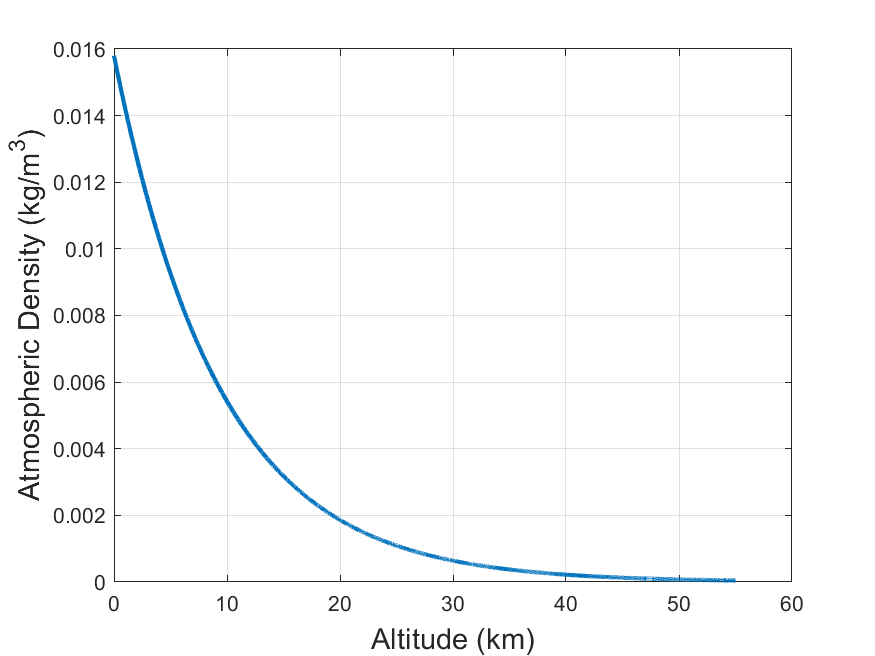
\includegraphics[width=1\textwidth]{Images/DensityNominal}
	\caption{The nominal atmospheric density.}
	\label{Fig:DensityNominal}
\end{figure}
\begin{figure}[h!]
	\centering
	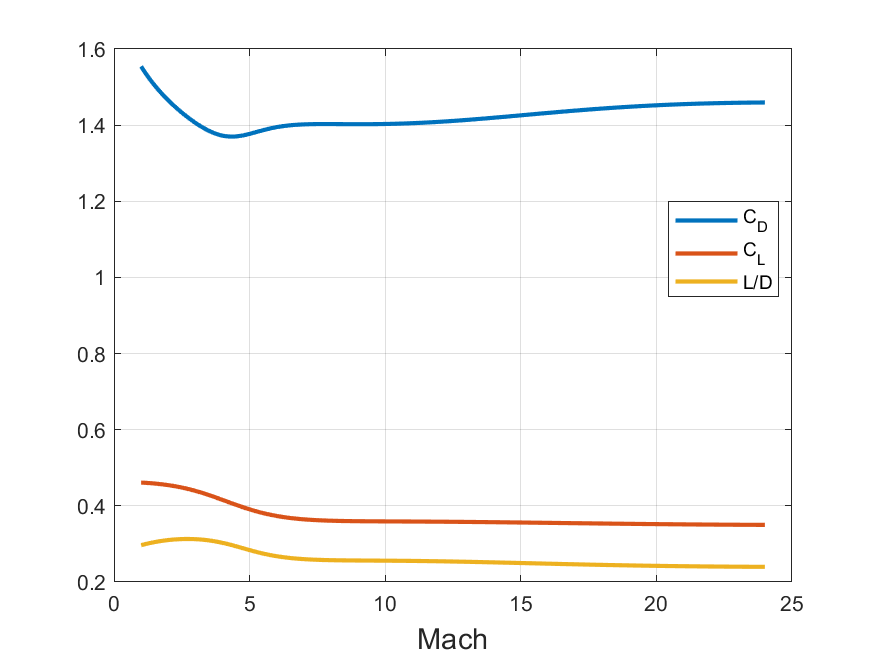
\includegraphics[width=1\textwidth]{Images/CoeffNominal}
	\caption{The nominal aerodynamic coefficients and $L/D$ profile.}
	\label{Fig:AeroCoeffNominal}
\end{figure}

\subsection{Uncertainty Models}
Typically, the uncertain initial state and model parameters are discussed in the context of assessing the guidance algorithm. However, in this dissertation, a key component of the guidance approach is incorporating uncertainty during the reference trajectory design, and thus they are given here. All uncertain variables are assumed to be normally distributed, but we note that the guidance approach developed in this dissertation applies to any distributed parameters with known mean and covariance. 

The approach phase, prior to the entry phase, targets a nominal entry state, but errors in the insertion maneuver and navigated state result in an uncertain entry state
\begin{align}
	\state(t_0, \delta\state_0) &= \bar{\state}_0 + \delta\state_0 \\
	\delta\state_0 &\sim \normal(\mathbf{0}, \cov_{\state_0}) \nonumber
\end{align}

Two key quantities in the study of entry vehicles are the lift-to-drag ratio, $L/D$, and ballistic coefficient, $\beta = \frac{m}{SC_D}$. Often, uncertainty is modeled in these values rather than in the aerodynamic coefficients, $C_L$ and $C_D$. For this reason, it is useful to rewrite Eqs.~(\ref{Eq:lift_accel})-(\ref{Eq:drag_accel}) in terms of these quantities and their uncertainties:
\begin{align}
	\begin{split}
		D &= \frac{1}{2}\frac{\rho}{\beta(1 + f_{\beta})} v^2 \\
		L &= D(\frac{L}{D})(1+f_{\frac{L}{D}})  \label{Eq:aero_accels}
	\end{split}
\end{align}
where $f_i\sim\normal(0, \sigma^2_i)$ are constant fractional offsets from the mean profile.
% i.e., $\delta\beta = \beta f_{\beta}$ and $\delta\frac{L}{D} = \frac{L}{D} f_{\frac{L}{D}}$.

Another key source of uncertainty in the entry dynamics is the atmospheric density model. The deviations are modeled as 
\begin{align}
	\rho(h) = \bar{\rho}(h) + f_{\rho}\delta\rho(h) \label{Eq:DensityUnc}
\end{align}
where $\bar{\rho}(h)$ is given by Eq.~\eqref{Eq:Density}. In Eq.~\eqref{Eq:DensityUnc}, the deviation $\delta\rho(h)$ is free to vary independently from the mean density. Note that this assumes that a constant fraction $f_{\rho}\sim\normal(0, \sigma^2_{\rho})$ of the standard deviation is applied throughout the trajectory. This can be used to bound the altitude-varying, possibly asymmetric density disturbances of models like MarsGRAM~\cite{MarsGRAM2010} or the Mars Climate Database (MCD)~\cite{MarsClimateDB}. See Fig.~\ref{Fig:DensityVariations} for an example where the boundary is determined by 1000 samples from the MCD~\cite{GuangfeiDissertation} and a symmetric model is created to bound the MCD model. Symmetry is required due to the Gaussian uncertainty assumption. 
\begin{figure}[h!]
	\centering
	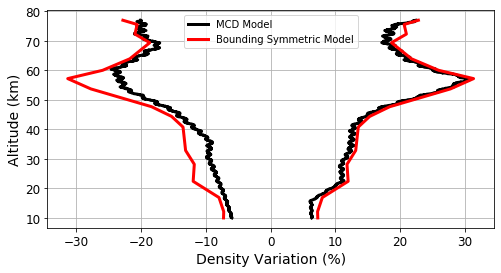
\includegraphics[width=0.9\textwidth]{Images/DensityVariations}
	\caption{Density variations from 1000 Mars Climate Database samples}
	\label{Fig:DensityVariations}
\end{figure} 

Collecting these uncertainties in the vector-valued random variable $\param = [\delta\state_0,\, f_{\frac{L}{D}},\, f_{\beta},\, f_{\rho}]^T$, the uncertain vehicle dynamics are written compactly as
\begin{align}
	\dot{\state}(t,\param) &= \dynamics(\state(t,\param), u(t,\state), \param),\quad
		\state(t_0,\param) = \state_0(\param) \label{Eq:UncertainDynamics}
\end{align}
where $\param \sim \mu = \normal(\mathbf{0},\cov_{\param})$ and 
\begin{align}
	\cov_{\param} = \begin{bmatrix}
		\cov_{\state_0} & & &\bigzero \\ 
		 &\sigma^2_{\frac{L}{D}} \\
		 & & \sigma^2_{\beta} \\
		\bigzero & & & \sigma^2_{\rho}
	\end{bmatrix}
\end{align}
%The domain and probability density function of the state vector vary with time. For this reason, the expected value is taken with respect to $\param$ throughout this dissertation. By the law of the unconscious statistician, 
%\begin{align}
%	\E{x(t,\param)} = \int_{\mathbb{R}^{n_p}}x(t,\param)\mu(\param)\mathrm{d}\param
%\end{align}
Note that, for a given realization of $\param$, the dynamics are a deterministic function of the state and control. A nominal trajectory is defined as one in which $\param=\mathbf{0}$. For nonlinear systems like the entry dynamics, the mean trajectory is not generally equal to the nominal trajectory, except at the initial time. 
The Taylor series of a generic scalar variable, $x(t,\param)$, expanded around $\param=\mathbf{0}$, is 
\begin{align}
	x(t,\param) = x(t,\mathbf{0}) + \Phi_1\param + \frac{1}{2}\param^T\Phi_2\param + \dots
\end{align} 
where $\Phi_i,\,i=1,2,3,\dots$ are the $i^{\mathrm{th}}$ partial derivatives of $x$. 
Truncating the series at second order and taking the expectation yields
\begin{align}
	\E{x(t,\param)} &= \E{x(t,\mathbf{0}) + \Phi_1\param + \frac{1}{2}\param^T\Phi_2\param} \\
	 &= x(t,\mathbf{0}) + \E{\frac{1}{2}\param^T\Phi_2\param}
\end{align}
where the second line follows from the linearity of the expectation operator and $\E{\param} = \mathbf{0}$. This latter fact also means $\cov_{\param} = V[\param] = \E{\param\param^T}$. 
The trace is also a linear function, so the expectation and trace can be swapped, i.e., $\E{\trace(A)} = \trace(\E{A})$. Together with the identity $\param^TA\param = \trace(A\param\param^T)$, we arrive at
\begin{align}
	 	\E{x(t,\param)} &= x(t,\mathbf{0}) + \frac{1}{2}\trace(\Phi_2\cov_{\param}) \label{Eq:TaylorExp}
\end{align}
From Eq.\eqref{Eq:TaylorExp} it can be seen that the nominal trajectory provides a first-order estimate of the mean. 
%We remark that a number of technical conditions on both the function $\dynamics$ (convergence of the Taylor series to the function) and the distribution of the random variable $\param$ (existence of higher moments, strong concentration) are required for the validity of the above Taylor series expansion analysis. However, this result is presented purely for analysis, and the numerical solution method presented later does not make use of it.
%TODO: rewrite this last part, maybe move it up. 



%%% Local Variables: ***
%%% mode: latex ***
%%% TeX-master: "thesis.tex" ***
%%% End: ***
